\documentclass[tikz,border=8pt]{standalone}
% Shared look for every TikZ diagram. Load with % Shared look for every TikZ diagram. Load with % Shared look for every TikZ diagram. Load with \input{../../tools/tikz-style.tex}
\usepackage[T1]{fontenc}
\usepackage{lmodern}
\renewcommand{\sfdefault}{lmr}  % diagrams use the same serif as the text
\usetikzlibrary{arrows.meta, positioning, shapes.geometric, calc, fit, backgrounds}
\definecolor{cblue}{HTML}{4C78A8}
\definecolor{corange}{HTML}{F58518}
\definecolor{cgreen}{HTML}{54A24B}
\definecolor{cred}{HTML}{E45756}
\definecolor{cpurple}{HTML}{B279A2}
\definecolor{cgrey}{HTML}{6B6B6B}
\tikzset{
  every picture/.style={font=\sffamily, line width=1.2pt},
  box/.style={draw=#1, fill=#1!12, rounded corners=4pt, align=center, inner sep=7pt, minimum height=1.1cm},
  box/.default=cgrey,
  arrow/.style={-{Stealth[length=3mm]}, draw=cgrey, line width=1.4pt},
  title/.style={font=\sffamily\bfseries\Large},
  note/.style={font=\sffamily\small, text=cgrey, align=center},
}
\AtBeginDocument{\hyphenpenalty=10000 \exhyphenpenalty=10000}

\usepackage[T1]{fontenc}
\usepackage{lmodern}
\renewcommand{\sfdefault}{lmr}  % diagrams use the same serif as the text
\usetikzlibrary{arrows.meta, positioning, shapes.geometric, calc, fit, backgrounds}
\definecolor{cblue}{HTML}{4C78A8}
\definecolor{corange}{HTML}{F58518}
\definecolor{cgreen}{HTML}{54A24B}
\definecolor{cred}{HTML}{E45756}
\definecolor{cpurple}{HTML}{B279A2}
\definecolor{cgrey}{HTML}{6B6B6B}
\tikzset{
  every picture/.style={font=\sffamily, line width=1.2pt},
  box/.style={draw=#1, fill=#1!12, rounded corners=4pt, align=center, inner sep=7pt, minimum height=1.1cm},
  box/.default=cgrey,
  arrow/.style={-{Stealth[length=3mm]}, draw=cgrey, line width=1.4pt},
  title/.style={font=\sffamily\bfseries\Large},
  note/.style={font=\sffamily\small, text=cgrey, align=center},
}
\AtBeginDocument{\hyphenpenalty=10000 \exhyphenpenalty=10000}

\usepackage[T1]{fontenc}
\usepackage{lmodern}
\renewcommand{\sfdefault}{lmr}  % diagrams use the same serif as the text
\usetikzlibrary{arrows.meta, positioning, shapes.geometric, calc, fit, backgrounds}
\definecolor{cblue}{HTML}{4C78A8}
\definecolor{corange}{HTML}{F58518}
\definecolor{cgreen}{HTML}{54A24B}
\definecolor{cred}{HTML}{E45756}
\definecolor{cpurple}{HTML}{B279A2}
\definecolor{cgrey}{HTML}{6B6B6B}
\tikzset{
  every picture/.style={font=\sffamily, line width=1.2pt},
  box/.style={draw=#1, fill=#1!12, rounded corners=4pt, align=center, inner sep=7pt, minimum height=1.1cm},
  box/.default=cgrey,
  arrow/.style={-{Stealth[length=3mm]}, draw=cgrey, line width=1.4pt},
  title/.style={font=\sffamily\bfseries\Large},
  note/.style={font=\sffamily\small, text=cgrey, align=center},
}
\AtBeginDocument{\hyphenpenalty=10000 \exhyphenpenalty=10000}

\begin{document}
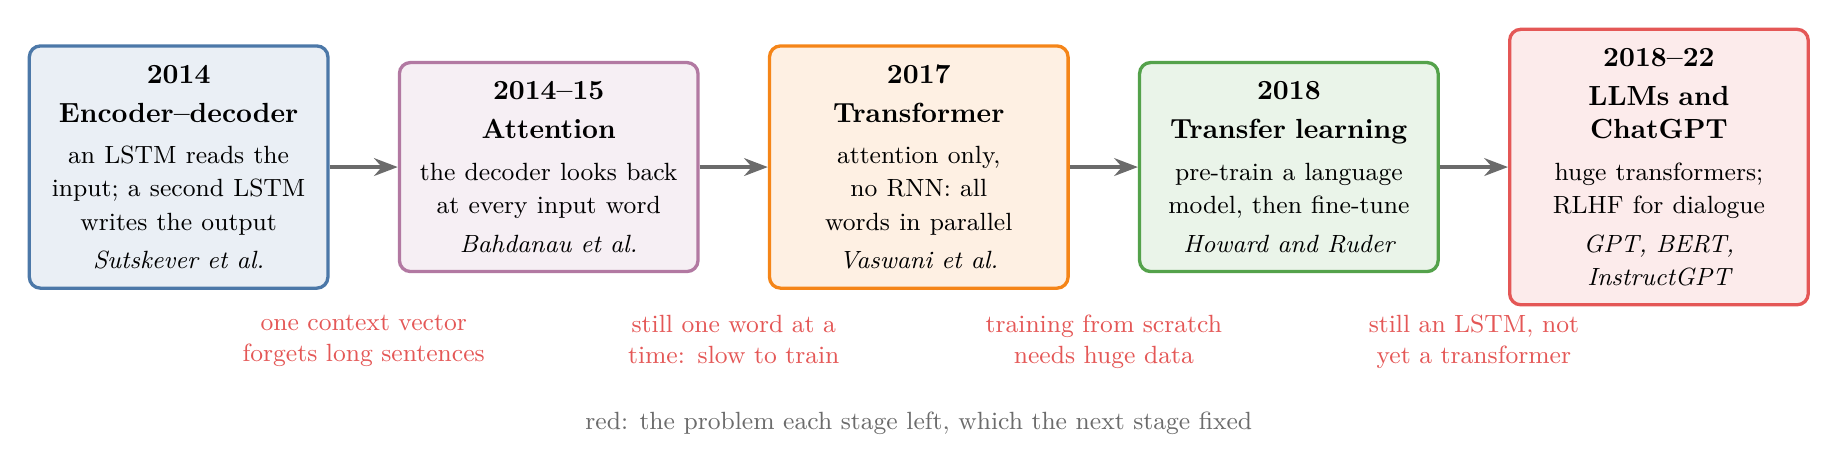
\begin{tikzpicture}[stage/.style={box=#1, text width=3.3cm, minimum height=2.3cm, font=\sffamily},
  prob/.style={font=\sffamily\small, text=cred, align=center, text width=3.1cm}]
  \foreach \i/\c/\yr/\name/\idea/\who in {
    1/cblue/2014/{Encoder--decoder}/{an LSTM reads the input; a second LSTM writes the output}/{Sutskever et al.},
    2/cpurple/2014--15/{Attention}/{the decoder looks back at every input word}/{Bahdanau et al.},
    3/corange/2017/{Transformer}/{attention only, no RNN: all words in parallel}/{Vaswani et al.},
    4/cgreen/2018/{Transfer learning}/{pre-train a language model, then fine-tune}/{Howard and Ruder},
    5/cred/2018--22/{LLMs and ChatGPT}/{huge transformers; RLHF for dialogue}/{GPT, BERT, InstructGPT}} {
    \node[stage=\c] (s\i) at (4.7*\i, 0) {\textbf{\yr}\\[2pt]\textbf{\name}\\[3pt]{\small \idea}\\[2pt]{\small\itshape \who}};
  }
  \foreach \i/\j in {1/2, 2/3, 3/4, 4/5} \draw[arrow] (s\i.east) -- (s\j.west);
  \foreach \x/\txt in {7.05/{one context vector forgets long sentences}, 11.75/{still one word at a time: slow to train}, 16.45/{training from scratch needs huge data}, 21.15/{still an LSTM, not yet a transformer}}
    \node[prob, anchor=north] at (\x, -1.75) {\txt};
  \node[note] at (14.1, -3.25) {red: the problem each stage left, which the next stage fixed};
\end{tikzpicture}
\end{document}
